\section{Hypothesis} \label{hypothesis} 

The hypothesis depicted in Figure \ref{fig:hypothesis}: \nameref{fig:hypothesis} proposes
that applying both Clean Architecture and Normalized Systems Theorems to a software
architecture leads to a modular software architecture that mitigates combinatorial
effects. Additionally, the hypothesis proposes improved stability and evolvability of
the C\# Software artifact, that is comparable with the result when using Java Software
artifacts \parencites[]{oorts_building_2014, de_bruyn_enabling_2018}.

\begin{figure}[!h]
    \centering
    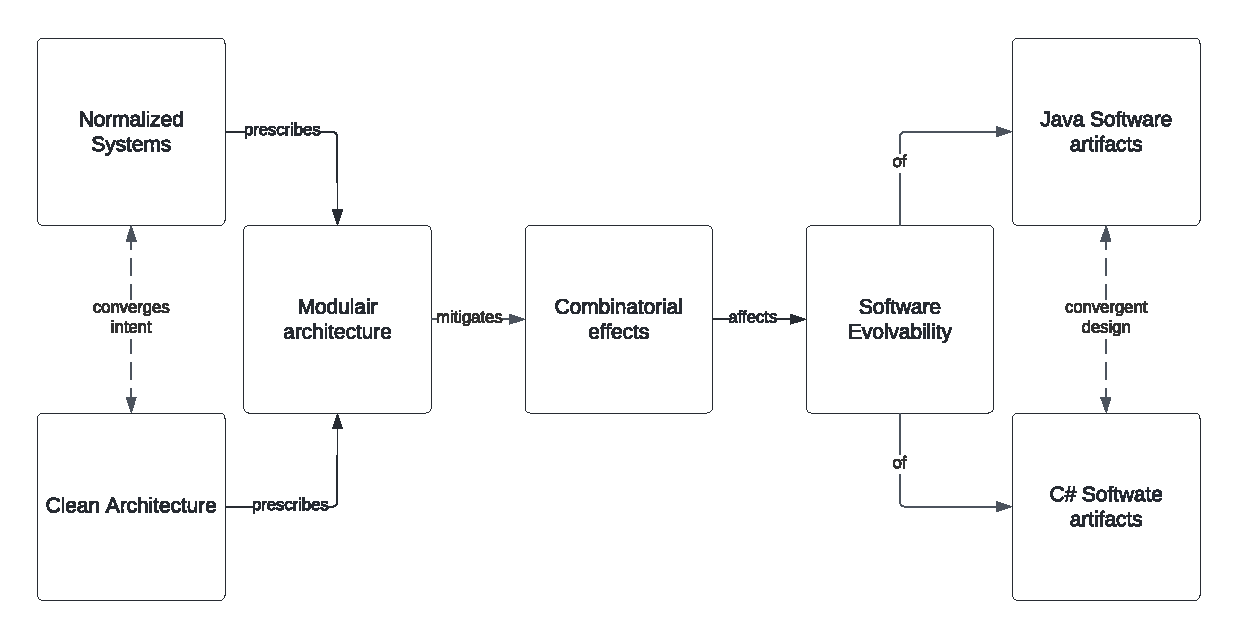
\includegraphics[width=1\textwidth]{Figures/hypothesis.pdf}
    \caption[The hypothesis]{The hypothesis}
    \label{fig:hypothesis}
\end{figure}